\chapter{Terminology} % Depth 0

\begin{itemize}
\item \textred{ADSL} : Asymmetric Digital Subscriber Line (high download speed but low upload speed).
\item \textred{ARP} : Address Resolution Protocol.
\item \textred{BPDU} : Bridge Protocol Data Unit.
\item \textred{CRC} : Cyclical Redundancy Check.
\item \textred{DNS} : Domain Name System. Naming system for associating various information (such as an IP address) with a domain name.
\item \textred{HTTP} : HyperText Transfer Protocol.
\item \textred{IEEE} : Institute of Electrical and Electronics Engineers.
\item \textred{LAN} : Local Area Network.
\item \textred{MSL} : Maximum Segment Life.
\item \textred{MTU} : Maximum Transmission Unit Maximum size of a protocol data unit that can be communicated in a single network layer transaction.
	\begin{itemize}
	\item \textred{Path MTU} : MTU size on the network between two Internet Protocol hosts.
	\end{itemize}
\item \textred{PDU} : Protocol data unit. Information that is transmitted as a single unit among peer entities of a computer network.
\item \textred{SDU} : Service Data Unit.
\item \textred{TLV} : Type-Length-Value. Encoding scheme used for optional information elements in a certain protocol. The first byte is a type, the second byte is the size of the value field and the rest is the value field.
\item \textred{DIFS} : DCF Interframe Space. If a station detects the medium has been continuously idle for a duration of DIFS, and the last frame transmission was successful (no corruption or error), it is then allowed to transmit a frame. If the last transmission contained an error, the station must wait for a duration of \textblue{EIFS} for any frame (re)transmission. DIFS respects the following relation : DIFS = \textblue{SIFS} + (2 * Slot time).
\item \textred{EIFS} : Extended Interframe Space. Similar to DIFS but is only activated if the last frame contains an error. The EIFS duration is defined as follows : Transmission time of Ack frame at lowest physical rate (or bit rate) + \textblue{SIFS} + \textblue{DIFS}.
\item \textred{SIFS} : Short Interframe Space. Amount of time in microseconds required for a wireless interface to process a received frame and to respond with a response frame. More precisely, it is the time interval between the last bit of the transmitted frame and the first bit of the corresponding response frame.
\item \textred{RIFS} : Reduced Interframe Space.
\end{itemize}

\chapter{Layers}

The reference model used is a simplified version of the OSI reference model (which contains 7 layers). This simplified model is divided into 5 layers :
\begin{itemize}
\item Physical
\item Datalink (LAN)
\item Network (WAN)
\item Transport (TCP/UDP)
\item Application (Web/mail)
\end{itemize}

\begin{figure}[H]
\centering
\scalebox{0.64}{
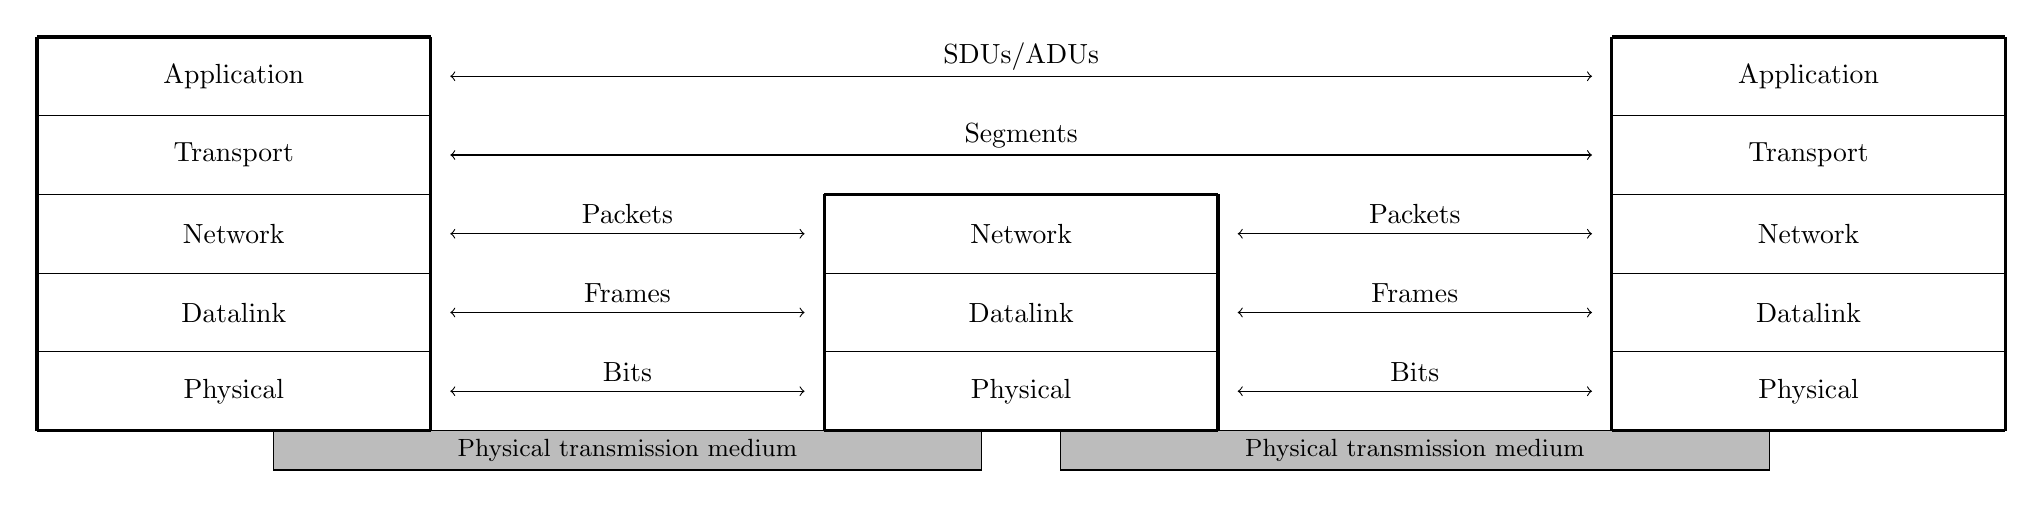
\begin{tikzpicture}
	\pgfdeclarelayer{nodelayer}
	\pgfdeclarelayer{edgelayer}
	\pgfsetlayers{edgelayer, nodelayer, main}
	\begin{pgfonlayer}{nodelayer}
		\node (0) at (0, 0) {};
		\node (1) at (0, -0.5) {};
		\node (2) at (2, 0) {};
		\node (3) at (2, 1) {};
		\node (4) at (-3, 0) {};
		\node (5) at (-3, 1) {};
		\node (6) at (7, 0) {};
		\node (8) at (7, 1) {};
		\node (9) at (12, 1) {};
		\node (10) at (12, 0) {};
		\node (11) at (9, -0.5) {};
		\node (12) at (9, 0) {};
		\node (13) at (10, 0) {};
		\node (14) at (10, -0.5) {};
		\node (15) at (17, 0) {};
		\node (16) at (17, 1) {};
		\node (17) at (19, 0) {};
		\node (18) at (19, -0.5) {};
		\node (19) at (22, 1) {};
		\node (20) at (22, 0) {};
		\node (21) at (7, 2) {};
		\node (22) at (7, 3) {};
		\node (23) at (12, 3) {};
		\node (24) at (12, 2) {};
		\node (25) at (-3, 2) {};
		\node (26) at (-3, 3) {};
		\node (27) at (2, 3) {};
		\node (28) at (2, 2) {};
		\node (29) at (2, 4) {};
		\node (30) at (2, 5) {};
		\node (31) at (-3, 5) {};
		\node (32) at (-3, 4) {};
		\node (33) at (17, 2) {};
		\node (34) at (17, 3) {};
		\node (35) at (17, 4) {};
		\node (36) at (22, 4) {};
		\node (37) at (22, 3) {};
		\node (38) at (22, 2) {};
		\node (39) at (17, 5) {};
		\node (40) at (22, 5) {};
		\node (41) at (14.5, -0.25) {\small Physical transmission medium};
		\node (45) at (4.5, -0.25) {\small Physical transmission medium};
		\node (46) at (-0.5, 0.5) {Physical};
		\node (47) at (-0.5, 1.5) {Datalink};
		\node (48) at (-0.5, 2.5) {Network};
		\node (49) at (-0.5, 3.5) {Transport};
		\node (50) at (-0.5, 4.5) {Application};
		\node (51) at (9.5, 2.5) {Network};
		\node (52) at (9.5, 1.5) {Datalink};
		\node (53) at (9.5, 0.5) {Physical};
		\node (54) at (19.5, 0.5) {Physical};
		\node (55) at (19.5, 1.5) {Datalink};
		\node (56) at (19.5, 2.5) {Network};
		\node (57) at (19.5, 3.5) {Transport};
		\node (58) at (19.5, 4.5) {Application};
		\node (59) at (2.25, 4.5) {};
		\node (60) at (16.75, 4.5) {};
		\node (61) at (2.25, 3.5) {};
		\node (62) at (16.75, 3.5) {};
		\node (63) at (2, 3) {};
		\node (64) at (2.25, 2.5) {};
		\node (65) at (6.75, 2.5) {};
		\node (66) at (2.25, 1.5) {};
		\node (67) at (6.75, 1.5) {};
		\node (68) at (2.25, 0.5) {};
		\node (69) at (6.75, 0.5) {};
		\node (70) at (12.25, 0.5) {};
		\node (71) at (16.75, 0.5) {};
		\node (72) at (12.25, 1.5) {};
		\node (73) at (16.75, 1.5) {};
		\node (74) at (12.25, 2.5) {};
		\node (75) at (16.75, 2.5) {};
		\node (76) at (9.5, 4.75) {SDUs/ADUs};
		\node (78) at (9.5, 3.75) {Segments};
		\node (79) at (4.5, 2.75) {Packets};
		\node (80) at (4.5, 1.75) {Frames};
		\node (81) at (4.5, 0.75) {Bits};
		\node (82) at (14.5, 0.75) {Bits};
		\node (84) at (14.5, 1.75) {Frames};
		\node (85) at (14.5, 2.75) {Packets};
	\end{pgfonlayer}
	\begin{pgfonlayer}{edgelayer}
		\draw [-, fill={rgb,255: red,188; green,188; blue,188}] (11.center)
			 to (1.center)
			 to (0.center)
			 to (12.center)
			 to cycle;
		\draw [-, fill={rgb,255: red,188; green,188; blue,188}] (14.center)
			 to (13.center)
			 to (17.center)
			 to (18.center)
			 to cycle;
		\draw [-, very thick] (20.center) to (40.center);
		\draw [-, very thick] (40.center) to (39.center);
		\draw [-, very thick] (39.center) to (15.center);
		\draw [-, very thick] (15.center) to (20.center);
		\draw [-, thin] (16.center) to (19.center);
		\draw [-, thin] (33.center) to (38.center);
		\draw [-, thin] (34.center) to (37.center);
		\draw [-, thin] (35.center) to (36.center);
		\draw [-, very thick] (2.center) to (30.center);
		\draw [-, very thick] (30.center) to (31.center);
		\draw [-, very thick] (31.center) to (4.center);
		\draw [-, very thick] (4.center) to (2.center);
		\draw [-, thin] (5.center) to (3.center);
		\draw [-, thin] (25.center) to (28.center);
		\draw [-, thin] (26.center) to (27.center);
		\draw [-, thin] (32.center) to (29.center);
		\draw [-, very thick] (6.center) to (10.center);
		\draw [-, very thick] (10.center) to (23.center);
		\draw [-, very thick] (23.center) to (22.center);
		\draw [-, very thick] (22.center) to (6.center);
		\draw [-, thin] (21.center) to (24.center);
		\draw [-, thin] (8.center) to (9.center);
		\draw [<->] (59.center) to (60.center);
		\draw [<->, in=180, out=0] (61.center) to (62.center);
		\draw [<->] (64.center) to (65.center);
		\draw [<->] (74.center) to (75.center);
		\draw [<->, in=180, out=0] (66.center) to (67.center);
		\draw [<->] (68.center) to (69.center);
		\draw [<->] (72.center) to (73.center);
		\draw [<->] (70.center) to (71.center);
	\end{pgfonlayer}
\end{tikzpicture}
}
\caption{The five layers reference model}
\end{figure}

\section{Physical Layer}

Here, we will see it only as a black bow which changes the value of a bit (because of electromagnetic interference) and which delivers more or fewer bits than requested (because of an imprecise clock frequency).

\section{Datalink Layer}

The Datalink layer allows two hosts that are directly connected through the physical layer to exchange information using \textblue{frames} (finite sequence of bits with a particular syntax or structure) on MAC addresses. 

When the Datalink layer entity needs to transmit a frame, it issues as many Data.request primitives to the underlying physical layer as there are bits in the frame. The physical layer will then convert the sequence of bits that will be sent over the physical medium. The receiver's physical layer will decode the received signal, recover the bits and issue the corresponding Data.indication primitives to its Datalink layer entity. If there are no transmission errors, this entity will receive the frame sent earlier.

A frame can be separated into 3 parts :
\begin{enumerate}
\item \textgreen{Header} : contains a flags to indicate its type (ACK, DATA) a sequence number and the length of the payload if there is one.
\item \textgreen{Payload} : contains the information that needs to be transmitted.
\item \textgreen{Error-detecting code} : allow the receiver to detect transmission errors. It is either a Hamming code, a Checksum, a Cyclic Redundancy Check (CRC), or a hash function.
\end{enumerate}

When transmitting a frame between switches, the packet stays the same. But when reaching a router, it will replace the addresses contained in the frame by its addresses.

\newpage
\section{Network Layer}

The network layer allows to exchange information between hosts that are not attached to the same physical medium using \textblue{packets}.

A packet is a finite sequence of bytes that is transported by the Datalink layer inside one or more frames. A packet usually contains information about its origin and its destination, and usually passes through devices on its way from its origin to its destination.

\section{Transport Layer}

Different communication flows can take place between the same hosts, they might have different needs and need to be distinguished. The transport layer ensures an identification of a communication flow between two given hosts using \textblue{segments}.

A segment is a finite sequence of bytes that are transported inside one or more packets. They are issued by the transport layer as Data.request to the underlying network layer entity.

They are different types of transport layers, the most widely used are :
\begin{itemize}
\item \textred{TCP} (Transmission Control Protocol) : provides a reliable connection-oriented bytestream transport service.
\item \textred{UDP} (User Datagram Protocol) : provides an unreliable connection-less transport service.
\end{itemize}

\section{Application}

The application layer includes all the mechanisms and data structure that are necessary for the applications.

Two application layers entities exchange data using generic \textblue{SDU} (Service Data Unit) or \textblue{ADU} (Application Data Unit) terms.

\chapter{Protocols}

\section{Datalink Layer}

\subsection[STP]{Spanning Tree Protocol (STP)}

Allows for reducing the network to a \textblue{Spanning Tree}.

\begin{minipage}{0.38\textwidth}
	\begin{figure}[H]
		\centering
		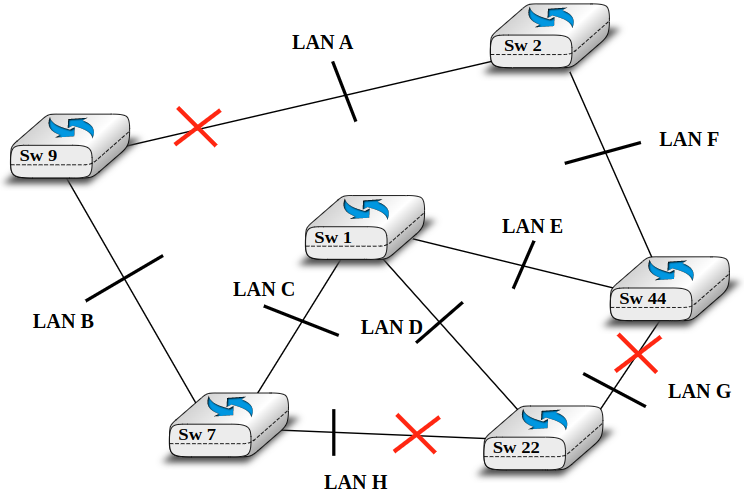
\includegraphics[width=0.9\textwidth,keepaspectratio]{stp_example}
		\caption{Spanning Tree example}
	\end{figure}
\end{minipage}
\begin{minipage}{0.6\textwidth}
	Switches running the Spanning Tree Protocol exchange BPDUs (\textblue{Bridge Protocol Data Unit}) that are always sent as frames. Each switch has a unique 64 bit identifier. The switches exchange BPDUs to build the spanning tree.
	
	Intuitively, the spanning tree is built by first selecting the switch with the smallest identifier as the root of the tree. The branches of the spanning tree are then composed of the shortest paths that allow all of the switches that compose the network to be reached.
\end{minipage}

The BPDU $:= \langle$ \textgreen{$R$}, \textgreen{$c$}, \textgreen{$T$}, \textgreen{$p$} $\rangle$ contains :
\begin{itemize}
\item The identifier of the \textgreen{root switch} ($R$)
\item The \textgreen{cost of the shortest path} between the switch that sent the BPDU and the root ($c$)
\item The identifier of the \textgreen{switch that sent} the BPDU ($T$)
\item The number of the \textgreen{switch port} over which the BPDU was sent ($P$)
\end{itemize}

The construction of the spanning tree depends on an ordering relationship among the BPDUs. This ordering relationship could be implemented by the following Python function :

\begin{minted}[frame=single,framesep=5pt,rulecolor=gray]{python}
# returns True if bpdu b1 is better than bpdu b2
def better(b1, b2):
    return ((b1.R < b2.R) or
            ((b1.R == b2.R) and (b1.c < b2.c)) or
            ((b1.R == b2.R) and (b1.c == b2.c) and (b1.T < b2.T)) or
            ((b1.R == b2.R) and (b1.c == b2.c) and (b1.T == b2.T) and (b1.p < b2.p)))
\end{minted}

A switch port can be in three different states : \textblue{Root}, \textgreen{Designated}, and \textred{Blocked}. All the ports of the root switch are in the Designated state.

The state of the ports on the other switches are determined as follow :
\begin{enumerate}
\item Each switch listens to BPDUs on its ports.
\item For every received BPDUs, the priority vector $V[q] = \langle R, c + cost(q), T, p, q \rangle$ (where $cost(q)$ is the cost associated to the port $q$ over which the BPDU was received) is computed and the best for each port is stored.
\item The root switch is found by looking at the smallest identifier in the priority vector table :
	\begin{itemize}
	\item The root switch at $\langle R, 0, R, p \rangle$ (where $R$ is the switch identifier and $p$ will be set to the port number over which the BPDU is sent).
	\item The other switches at $\langle R, c', S, p \rangle$ (where $R$ is the root identifier, $c'$ the cost of the best root priority vector, $S$ the identifier of the switch and $p$ will be replaced by the number of the port over which the BPDU will be sent) know their \textblue{Root} port (the one with the best priority vector).
	\end{itemize}
\item A port is \textgreen{Designated} if the switch's BPDU is better than the port’s priority vector, otherwise it is \textred{Blocked}.
\end{enumerate}

\section{Network Layer}

\subsection[IPv6]{Internet Protocol Version 6 (IPv6)}

Soon, IPv4 won't be able to accommodate for all addresses anymore, which is why another solution is needed.
IPv6 addresses are encoded on 128 bits ($3.4*10^{38}$ different IPv6 addresses), their format header can easily be parsed by hardware devices, they and can be configured automatically, and they provide more security.

\subsubsection{Textual representation of IPv6 addresses}

The preferred format for writing IPv6 addresses is \textcolor{pink}{x:x:x:x:x:x:x:x}, where the \textcolor{pink}{x}‘s are hexadecimal digits representing the eight 16-bit parts of the address. Example : \textcolor{pink}{abcd:ef01:2345:6789:abcd:ef01:2345:6789}.

\textcolor{pink}{::} is used to indicate one or more groups of 16 bits blocks containing only bits set to 0. Example : \textcolor{pink}{ff01:0:0:0:0:0:0:101} is represented as \textcolor{pink}{ff01::101}.

An IPv6 prefix can be represented as \textit{address}/\textit{length}, where \textit{length} is the length of the prefix in bits. Example : \textcolor{pink}{2001:0db8:0000:cd30:0000:0000:0000:0000}/\textcolor{pink}{60} == \textcolor{pink}{2001:0db8:0:cd30::}/\textcolor{pink}{60}.

\subsubsection{IPv6 addressing architecture}

The scalability of a network layer depends on its addressing architecture. IPv6 supports unicast, multicast and anycast architectures.

\paragraph{Unicast}

\begin{minipage}{0.55\textwidth}
	\begin{figure}[H]
	    \centering
	    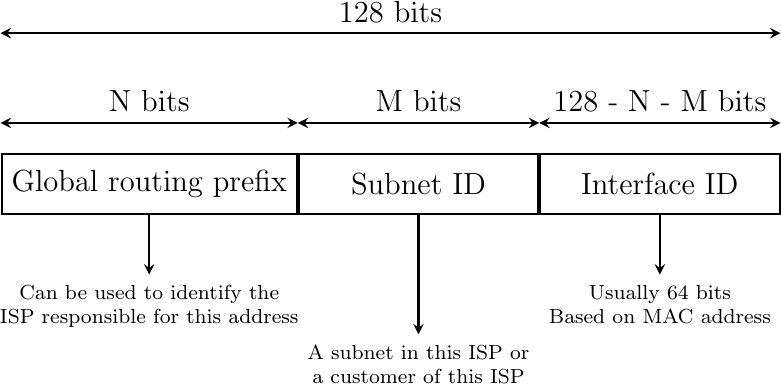
\includegraphics[width=0.9\textwidth,keepaspectratio]{unicast}
	    \caption{Structure of IPv6 unicast addresses}
	\end{figure}
\end{minipage}
\begin{minipage}{0.44\textwidth}
	An IPv6 unicast address is composed of three parts :
	\begin{enumerate}
	\item A \textred{global routing prefix} that is assigned to the Internet Service Provider that owns this block of addresses.
	\item A \textred{subnet identifier} that identifies a customer of the ISP.
	\item An \textred{interface identifier} that identifies a particular interface on a host.
	\end{enumerate}
\end{minipage}

To preserve the scalability of the routing system, it is important to minimize the number of routes that are stored on each router. Hierarchical address allocation allows for minimizing the amount of routes known to the router. It therefore only knows the route for certain address blocks ($2^{128}$ grouped in $2^{64}$ subnets).
Two types of address allocation:
\begin{itemize}
\item Provider-Independent (PI): For companies connected to at least two ISPs. Address blocks are given out independently of the ISP.
\item Provider-Aggregatable (PA): Depends on the ISP.
\end{itemize}

The drawback with PA addresses is that when your provider changes, all the addresses you use in a PA address block also change. The typical \textred{size of the IPv6 address} blocks are :
\begin{itemize}
\item /\textcolor{pink}{32} for an Internet Service Provider
\item /\textcolor{pink}{48} for a single company
\item /\textcolor{pink}{56} for small user sites
\item /\textcolor{pink}{64} for a single user (e.g. a home user connected via ADSL)
\item /\textcolor{pink}{128} in the rare case when it is known that no more than one host will be attached
\end{itemize}

The \textred{usage of the IPv6 prefix} is the following : the longest prefix match assures the route that has the best match with the address is the one that is used (\textcolor{pink}{::}/\textcolor{pink}{0} matches with all and is therefore the default route).

The \textred{Unique Local Unicast} (ULA) address is an \textcolor{pink}{fc00::/7} and is similar to an IPv4 address. The address isn’t necessarily unique and a router doesn’t forward a ULA. As opposed to local unicast links, it doesn’t necessarily need to have the same link.

\textred{Link Local Unicast} : the address starts with \textcolor{pink}{fe80::}/\textcolor{pink}{64}, followed by 64 interface bits. Used when two hosts on the same link (or LAN) want to exchange a packet. The router can’t forward a packet with a local unicast link. (Used when regular IPv6 isn’t an option, that is, an isolated LAN.)

\paragraph{Multicast}

Allows for sending a packet to all people in a same LAN group.

\begin{figure}[H]
    \centering
    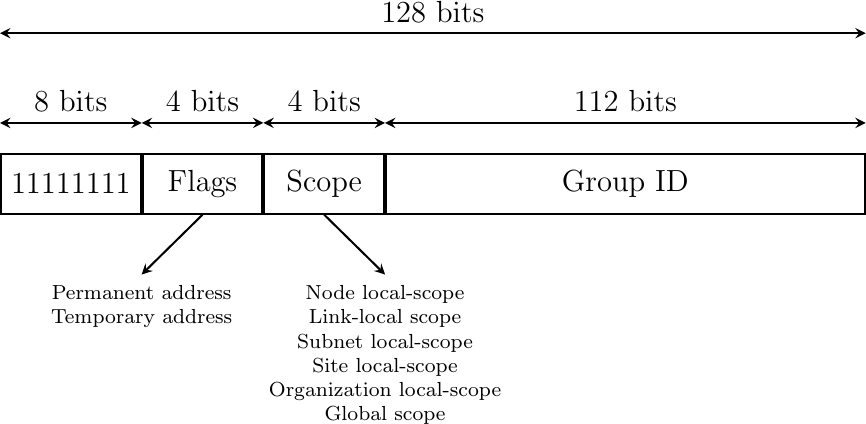
\includegraphics[width=0.5\textwidth,keepaspectratio]{multicast}
    \caption{IPv6 multicast address structure}
\end{figure}

\subsubsection{IPv6 packet format}

\begin{figure}[H]
    \centering
    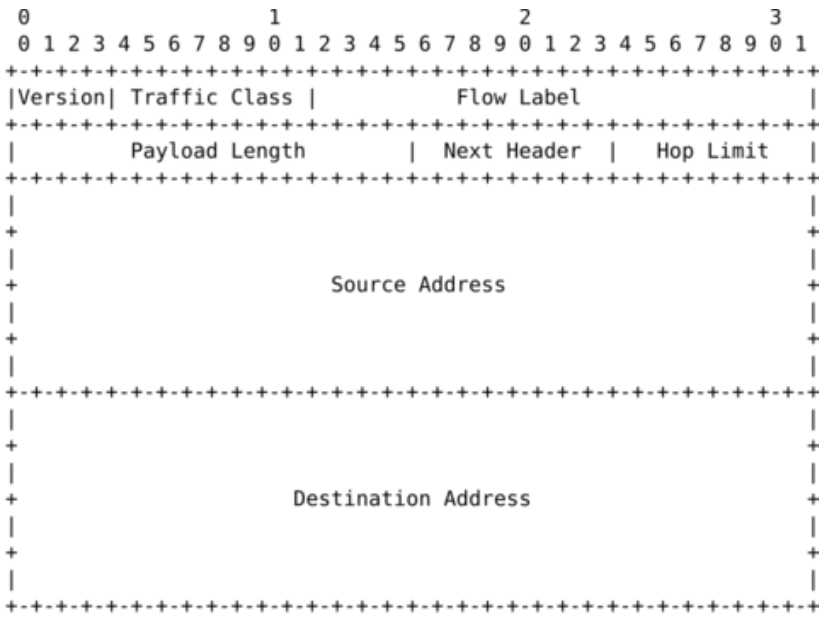
\includegraphics[width=0.4\textwidth,keepaspectratio]{ipv6_packet_format}
    \caption{IPv6 packet format}
\end{figure}

The Header field (40bits) is composed of Payload length (16bits, maximum $\approx 64kB$), Hop limit\footnote{When retransmitting a packet, the hop limit is decremented. When it reaches 0, the packet is dropped and a error is send to the source.} (8bits) and Next header (8bits) + Version (4bits) + SRC (128bits) + DST (128bits) + Traffic (8bits ECE/ECT).

The Next Header field identifies the encapsulated data (if UDP, TCP, etc.)

\subsection[ICMPv6]{Internet Control Message Protocol version 6 (ICMPv6)}

Internet Control Message Protocol version 6 is used in IPv6 packets to transmit messages to the sender (used mainly for debugging purposes). There are two types of messages:
\begin{itemize}
\item Error messages : Destination unreachable, Packet too big, Time exceeded, Parameter problem.
\item Information messages : when a host receives an Echo request, it has to respond with an Echo reply.
\end{itemize}

In order to do so, we will a 4 fields to the IPv6 packets : Type, Code, Checksum, Message Body.

\subsection{Intradomain routing}

\subsubsection[RIP]{Routing Information Protocol (RIP)}

The Routing Information Protocol (RIP) is the simplest routing protocol that was standardized for the TCP/IP protocol suite. RIP routers periodically exchange RIP messages sent inside a UDP segment.

\begin{minipage}{0.55\textwidth}
	\begin{figure}[H]
		\centering
		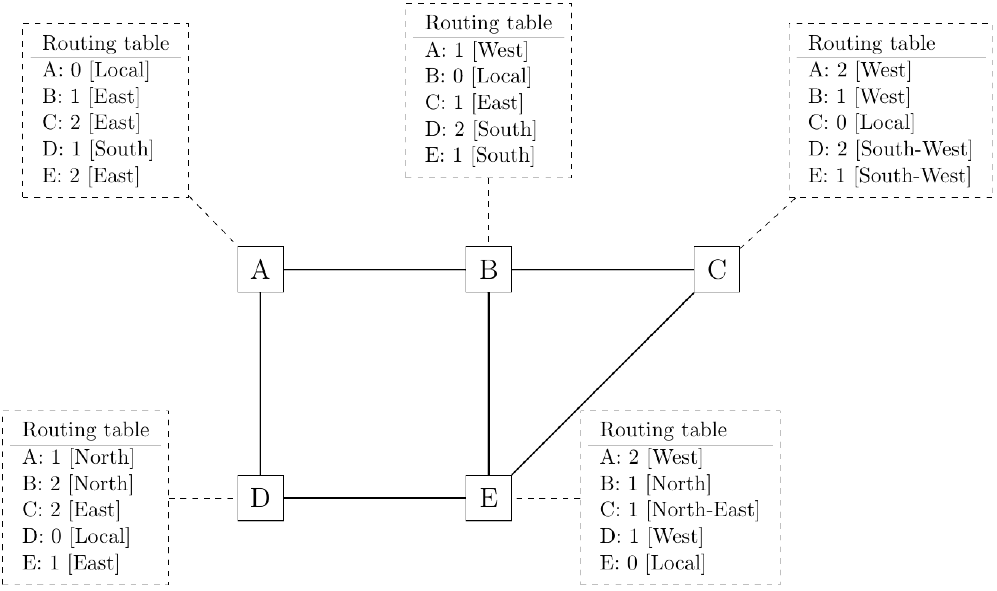
\includegraphics[width=\textwidth,keepaspectratio]{rip_example}
		\caption{Routing tables in RIP}
	\end{figure}
\end{minipage}
\begin{minipage}{0.44\textwidth}
	When a router boots, its routing table is empty and it cannot forward any packet. To speedup the discovery of the network, it can send a request message to the RIP IPv6 multicast address. All RIP routers listen to this multicast address and any router attached to the subnet will reply by sending its own routing table as a sequence of RIP messages. These messages contain the distance vectors that summarize the router’s \textblue{routing table}.
\end{minipage}

\subsubsection[OSPF]{Open Shortest Path First (OSPF)}

With link-state routing, it’s very costly for big networks to store all of the network in memory. To resolve this issue, we introduce hierarchical routing that divides the network into regions. In OSPF, a region is called an area.
OSPF uses the following terminology :

\begin{minipage}{0.38\textwidth}
	\begin{figure}[H]
		\centering
		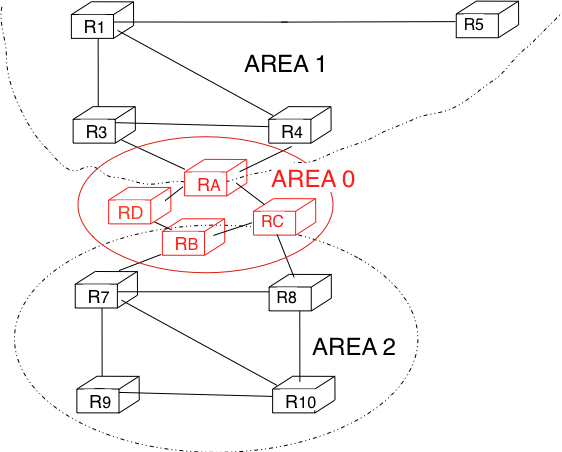
\includegraphics[width=\textwidth,keepaspectratio]{ospf-areas}
		\caption{OSPF areas}
	\end{figure}
\end{minipage}
\begin{minipage}{0.61\textwidth}
	\begin{itemize}
	\item \textblue{Area} : set of routers and links grouped together. Routers know the topology of their area and how to reach the backbone area, they exchange link-state packets with everyone in the area.
	\item \textblue{Backbone Area} : area that groups the border routers and those that aren’t in an area (\textred{AREA 0}).
	\item \textblue{Area border router} : router attached to several areas (RA, RB, RC).
	\item \textblue{Internal router} : router whose directly connected networks belong to the area.
	\end{itemize}
\end{minipage}

\paragraph*{Inter-area}

Inter-area routing is done by switching distance vector protocols to prevent routers from having additional costs to reach routers from a different domain.

\paragraph*{LAN}

When routers boot in a LAN, they elect a \textblue{Designated Router} (DR) so as to not have to exchange HELLO packets between all the routers. The routers can only exchange HELLOs with the DR; it represents the LAN.

\newpage
\subsection{Interdomain routing}

\subsubsection[BGP]{Border Gateway Protocol (BGP)}

In the Border Gateway Protocol, when en BGP router advertises a route towards a prefix, it announces the IP prefix and the interdomain path used to reach this prefix. As in BGP, every domain is identified by a unique \textred{Autonomous System} (AS) number, the interdomain path contains the AS numbers of the transit domains that are used to reach the associated prefix.

\begin{figure}[H]
	\centering
	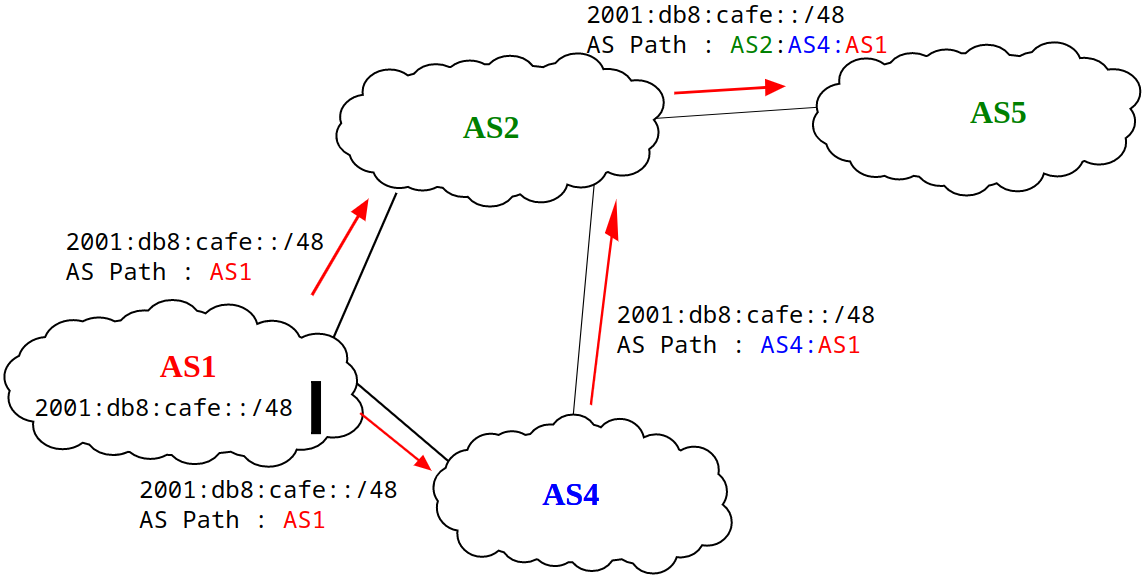
\includegraphics[width=0.6\textwidth,keepaspectratio]{bgp_example}
	\caption{Exchange of BGP routes}
\end{figure}

Example with the above BGP route : Thanks to the AS-Path, $AS5$ knows that if it sends a packet towards \textit{2001:db8:cafe::/48}, the packet first passes through $AS2$, then through $AS4$ before reaching its destination inside $AS1$.

A BGP route will rank each route that it as learned following its own ranking algorithm (i.e. each router will maximize its benefits) and will advertise the best one (is the above example, $AS2$ advertises the route it learned from $AS4$ rather than the other it learned from $AS1$).

\section{Transport Layer}

\subsection[UDP]{User Datagram Protocol (UDP)}

The User Datagram Protocol is used when delay must be minimized or losses can be recovered by the application itself (or real-time application like interactive videos). It is an unreliable connectionless transport service, running on top of an unreliable connectionless network service, which uses ports to allow communicating with multiple applications (errors are detected using the checksum).
\begin{figure}[H]
    \centering
    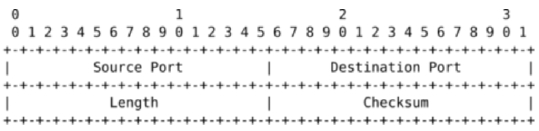
\includegraphics[width=0.4\textwidth,keepaspectratio]{udp_header}
    \caption{UDP header format}
\end{figure}

\subsection[TCP]{Transmission Control Protocol (TCP)}

The Transmission control protocol is a bidirectional bytestream of a \textred{connection-oriented} transport service running on top of an unreliable connectionless network service.
\begin{figure}[H]
    \centering
    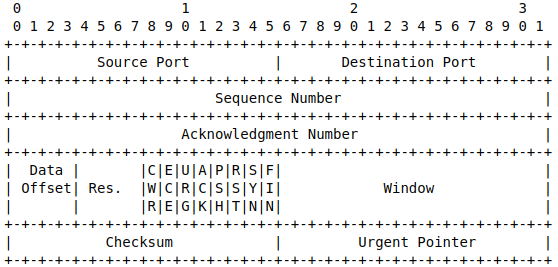
\includegraphics[width=0.3\textwidth,keepaspectratio]{tcp_header}
    \caption{TCP header format}
\end{figure}

\subsubsection{Connection establishment}

\begin{figure}[H]
    \centering
    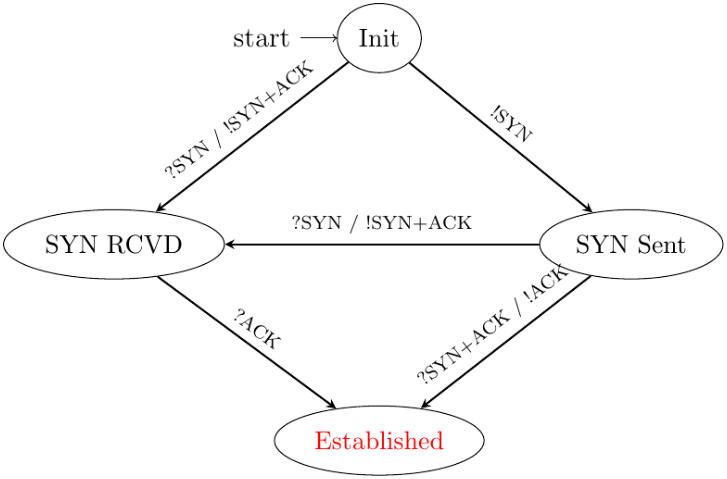
\includegraphics[width=0.4\textwidth,keepaspectratio]{three_way_handshake}\hfill	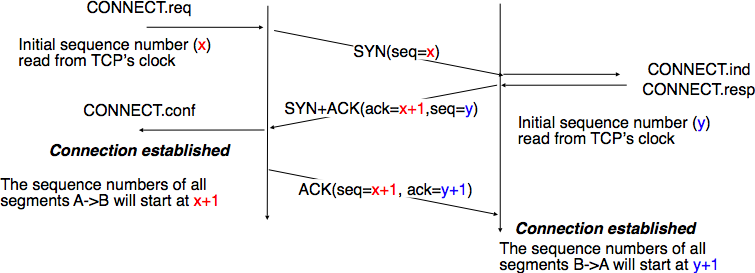
\includegraphics[width=0.6\textwidth,keepaspectratio]{tcp-estab}
	\caption{Three-way handshake}
\end{figure}

The Three-way handshake uses a sequence number, an acknowledgement number, and SYN/ACK/RST flags.
The different messages types in TCP are :
\begin{itemize}
\item Synchronize (SYN) : Used to initiate and establish a connection. It also helps you to synchronize sequence numbers between devices
\item Acknowledgement (ACK) : Helps to confirm to the other side that it has received the SYN
\item Synchronize+Acknowledgement (SYN+ACK) : SYN message from local device and ACK of the earlier packet
\item Reset (RST) : Used to signal a refused connection
\item FIN : Used to signal a connection release (end of transmission)
\end{itemize}

\subsubsection{Congestion control}

Network congestion describes the reduced quality of service that occurs when a network node is carrying more data that it can handle.

TCP controls congestion by acting on the window size since a connection can't send data faster than $\frac{window}{rtt}$ where $window$ is the maximum between the host's sending window and the window advertised by the receiver, and $rtt$ is the round-trip-time (delay between the transmission of a segment and the reception of an ack).

In general, the maximum throughput that can be achieved by a TCP connection depends on its maximum window size and the rtt if there are no losses. If there are losses, it depends on the MSS, the rtt and the loss ratio. This gives the following relation :
\begin{equation*}
Throughput < min(\frac{window}{rtt}, \frac{k * MSS}{rtt * \sqrt{p}})
\end{equation*}
Where :
\begin{itemize}
\item $k =$ a constant
\item $MSS =$ Maximum Segment Size (most hosts use the same $MSS = 1460B$)
\item $p =$ loss ratio
\end{itemize}

As we can see, TCP connections with smaller $rtt$ and/or a larger $MSS$ can achieve a higher throughput than other TCP connections (unfairness).

\newpage
The TCP congestion control scheme can be implemented using the following algorithm (also called \textit{AIMD congestion control}) :
\begin{minted}[frame=single,framesep=5pt,rulecolor=gray]{python}
# Initialization
cwnd = MSS  # congestion window in bytes
ssthresh= swin # in bytes

# Ack arrival
if tcp.ack > snd.una:  # new ack, no congestion
    if dupacks == 0:  # not currently recovering from loss
        if cwnd < ssthresh:
            # slow-start : quickly increase cwnd
            # double cwnd every rtt
            cwnd = cwnd + MSS
        else:
            # congestion avoidance : slowly increase cwnd
            # increase cwnd by one mss every rtt
            cwnd = cwnd + MSS * (MSS / cwnd)
    else:  # recovering from loss
        cwnd = ssthresh  # deflate cwnd RFC5681
        dupacks = 0
else:  # duplicate or old ack
    if tcp.ack == snd.una:  # duplicate acknowledgment
        dupacks += 1
        if dupacks == 1 or dupacks == 2:
            send_next_unacked_segment  # RFC3042
        if dupacks == 3:
            retransmitsegment(snd.una)
            ssthresh = max(cwnd/2, 2*MSS)
            cwnd = ssthresh
        if dupacks > 3:  # RFC5681
            cwnd = cwnd + MSS  # inflate cwnd
    else:
        # ack for old segment, ignored
        pass

Expiration of the retransmission timer:
    send(snd.una)  # retransmit first lost segment
    sshtresh = max(cwnd/2, 2*MSS)
    cwnd = MSS
\end{minted}

\newpage
\section{Application Layer}

\subsection{DNS}

The Domain Name System (DNS) protocol runs above the datagram and bytestream service. The header of DNS messages is divided into 5 parts. The first tree are mandatory (the other two are optional) and are :
\begin{itemize}
\item ID : each request is given an ID to verify that it is the correct DNS request (example : the request $foo$ will be given the $ID_{foo}$ and the request $bar$ will be given the $ID_{bar}$ and will not conflict when the response is send)
\item Flag Recursive : Used to know if the DNS server will resolve the entire IP at once (the resolver recuses through the DNS hierarchy to retrieve its answer)
\item Flag Authority : Used to known wherever the response comes from a server cache or not
\end{itemize}

The command \textred{$dig$} can give retrieve the IP of e server (3 types of record : $A$ (IPv4), $AAAA$ (IPv6), and $MX$ (mail server). Example : If you want to retrieve the IP of a mail server :
\begin{minted}[frame=single,framesep=5pt,rulecolor=gray]{bash}
dig -t MX student.uclouvain.be +short
# student-uclouvain-be.mail.protected.outlook.com
COM=$(dig +short -t NS com | head -n 1)
OUT=$(dig +short @$COM -t NS outlook.com | head -n 1)
PRO=$(dig +short @$OUT -t NS protected.outlook.com | head -n 1)
MAI=$(dig +short @$PRO -t NS mail.protected.outlook.com | head -n 1)
dig +short @$PRO student-uclouvain-be.mail.protected.outlook.com | head -n 1
\end{minted}

\subsection{Mails}

An email system is composed of a :
\begin{itemize}
\item A message format
\item Protocols exchange between host and server
\item A client software to create/read mails
\item A software to allow the server to efficiently exchange mails.
\end{itemize}

\begin{figure}[H]
\centering
\scalebox{0.5}{
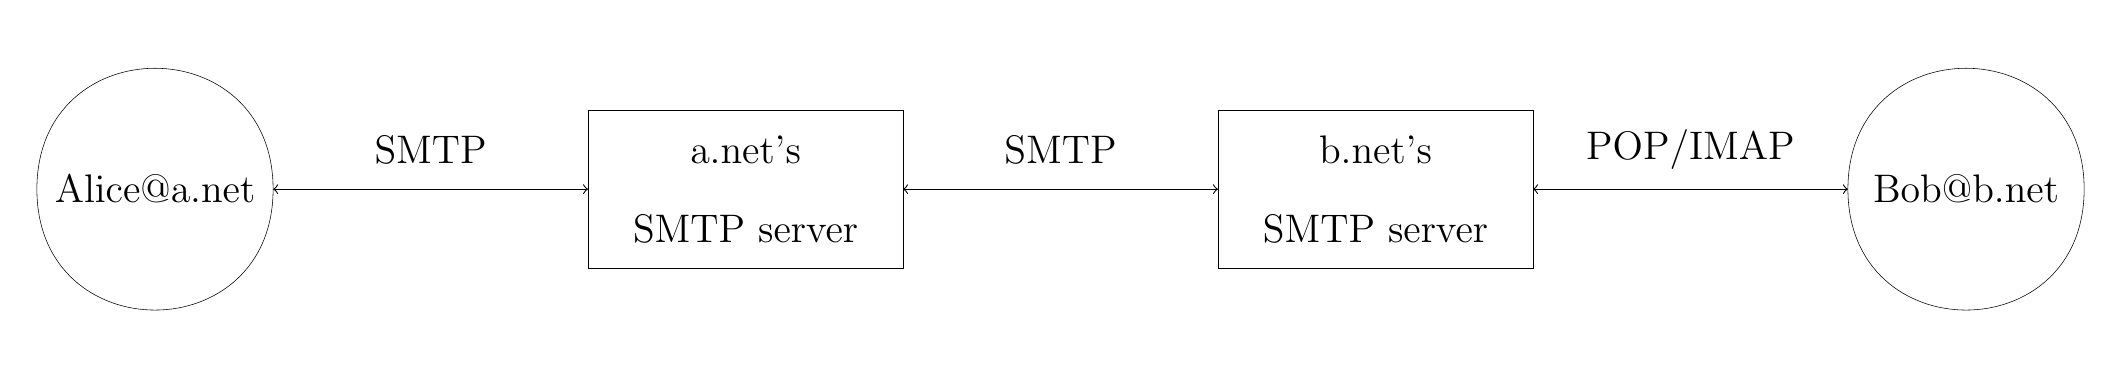
\begin{tikzpicture}
	\pgfdeclarelayer{nodelayer}
	\pgfdeclarelayer{edgelayer}
	\pgfsetlayers{edgelayer, nodelayer, main}
	\begin{pgfonlayer}{nodelayer}
		\node (0) at (-13, 0) {};
		\node (1) at (-10, 0) {};
		\node (2) at (-6, 0) {};
		\node (3) at (-2, 0) {};
		\node (4) at (2, 0) {};
		\node (5) at (6, 0) {};
		\node (6) at (10, 0) {};
		\node (7) at (13, 0) {};
		\node (8) at (-6, 1) {};
		\node (9) at (-2, 1) {};
		\node (10) at (-2, -1) {};
		\node (11) at (-6, -1) {};
		\node (12) at (2, 1) {};
		\node (13) at (6, 1) {};
		\node (14) at (6, -1) {};
		\node (15) at (2, -1) {};
		\node (16) at (-11.5, 0) {\Large Alice@a.net };
		\node (17) at (-4, 0.5) {\Large a.net's };
		\node (18) at (4, 0.5) {\Large b.net's };
		\node (19) at (11.5, 0) {\Large Bob@b.net };
		\node (20) at (-8, 0.5) {\Large \textred{SMTP}};
		\node (21) at (0, 0.5) {\Large \textred{SMTP} };
		\node (22) at (8, 0.5) {\Large \textblue{POP/IMAP}};
		\node (23) at (-4, -0.5) {\Large SMTP server };
		\node (24) at (4, -0.5) {\Large SMTP server };
	\end{pgfonlayer}
	\begin{pgfonlayer}{edgelayer}
		\draw [very thin] (1.center)
			 to [in=-90, out=-90, looseness=1.75] (0.center)
			 to [bend left=90, looseness=1.75] cycle;
		\draw [<->] (1.center) to (2.center);
		\draw [<->] (3.center) to (4.center);
		\draw [<->] (5.center) to (6.center);
		\draw [very thin] (7.center)
			 to [in=-90, out=-90, looseness=1.75] (6.center)
			 to [in=90, out=90, looseness=1.75] cycle;
		\draw [very thin] (14.center)
			 to (15.center)
			 to (12.center)
			 to (13.center)
			 to cycle;
		\draw [very thin] (8.center)
			 to (9.center)
			 to (10.center)
			 to (11.center)
			 to cycle;
	\end{pgfonlayer}
\end{tikzpicture}
}
\caption{Simplified mail architecture}
\end{figure}

Here, Alice sends a mail using $SMTP$ to her mail server. Bob will retrieve its mail either using $POP$ (removes it from the server) or using $IMAP$ (create a copy). These 3 protocols uses TCP.

\subsubsection{Simple Mail Transfer Protocol (SMTP)}

SMTP allows client to send emails and does not require authentication to be used. Each SMTP message send must contain: the (mail) address $from$, the (mail) address $to$ and a date.

\subsubsection{Post Office Protocol (POP) and Internet Message Access Protocol (IMAP)}

POP and IMAP allows client to retrieve their emails from a server. Both POP and IMAP require authentication to be used.

\begin{enumerate}
\item Establish a connection with the mail server
\item Authenticate the user
\item Downloads the mails from the server
\end{enumerate}

\subsubsection{Multipurpose Internet Mail Extensions (MIME)}

MIME was designed to allow email to carry non-ASCII characters and binary files without breaking the email servers that were deployed at that time. In order to do so, new header fields were added to support MIME (MIME-version, Content-type, and Content-Transfer-Encoding).

\subsection{HyperText Transfer Protocol (HTTP)}

To replace the File Transfer Protocol (FTP), the \textit{World Wide Web} was created using hupertext to link files together. The three components of the World Wild Web are :
\begin{enumerate}
\item \textred{Uniform Resource Identifier (URI)} that uniquely identifies a resource on the WWW. It is divided into three parts : '\textit{\textcolor{deepGreen}{protocol://}\textcolor{deepBlue}{user@server:port}\textcolor{orange}{/resource}}'
	\begin{enumerate}
	\item[\textcolor{deepGreen}{(a)}] A protocol for the application layer (http://, mailto:, ftp://)
	\item[\textcolor{deepBlue}{(b)}] Authority which is the IP address or DNS server where the file is located
	\item[\textcolor{orange}{(c)}] A path to the file in UNIX format
	\end{enumerate}
\item HTML : A standard document format (divided into two parts : header and body) containing hypertext link
\item HTTP : A standard protocol with efficient access to document on the server, made of request and responses. It contains :
	\begin{enumerate}
	\item A method (GET, HEAD, POST), a URI and a version of the HTTP
	\item A header (specifies optional parameters)
	\item An optional MIME document 
	\end{enumerate}
\end{enumerate}

\subsubsection{Comparisons}

HTTP evolved during its different versions :

\begin{table}[H]
	\centering
	\begin{tabular}{r|l|l}
	\hline 
	 & HTTP 1.0 & HTTP 1.1 \\ 
	\hline 
	TCP Connection & One per data & Persistent support (keep alive) \\ 
	\hline 
	Caching & If-Modified-Since & Based on an entity tag \\ 
	\hline 
	Host Header & No & Yes \\ 
	\hline 
	\end{tabular}
	\caption{TCP in HTTP 1.0 VS HTTP 1.1}
\end{table}

\begin{table}[H]
	\centering
	\begin{tabular}{r|l|l}
	\hline 
	 & HTTP 1.1 & HTTP 2.0 \\ 
	\hline 
	Encoding & ASCII & Binary \\ 
	\hline 
	Optimization method & Pipelining & Multiplexing \\ 
	\hline 
	Compression support & No & Yes \\ 
	\hline 
	Push support & No & Yes \\ 
	\hline 
	\end{tabular}
	\caption{TCP in HTTP 1.1 VS HTTP 2.0}
\end{table}

\subsection{Secure Shell (SSH)}

The Secure Shell runs directly above the TCP protocol and allows for remote logins. Each user possess a \textred{public and a private key}. When a message is send via SSH, it is send using the public key of the receiver that will be able to decrypt it using its private key.

Contrary to TLS, SSH does not require any certificate. As the algorithm takes into account the fact that the client's cache contains the public key of the server. This means that, in the case of a MITM (Man-In-The-Middle) attack, the protocol will see that the keys do not match and warn the user (which will decide to continue or not).

For a connection, there is simply an exchange where the client indicate its SSH version and where the server answers with its. Then, the client will communicate the encryption algorithm it knows and the server will answer with the one it will use.

\subsection{Transport Layer Security (TLS)}

The TLS family of protocols works basically the same way as SSH but instead of using private keys, it will use \textred{certificates}. This is due to the fact that, when navigation over a large number or pages, the client cannot store every public key it encounters. Instead of exchanging keys, the client/server will exchange digital certificates.
